\documentclass[12pt,fleqn]{article}
\usepackage{float}
\usepackage{blindtext}
\usepackage[en,bordered]{uni-style}
\usepackage{uni-math}
\usepackage{adjustbox}
\usepackage{fontspec}
\usepackage{listings}
\usepackage{color} %red, green, blue, yellow, cyan, magenta, black, white
\definecolor{mygreen}{RGB}{28,172,0} % color values Red, Green, Blue
\definecolor{mylilas}{RGB}{170,55,241}
\setmainfont{Crimson-Roman.ttf}
\title{Engineering Mathematics Project}
\prof{ Prof. Hamid K. Aghajan}
\subtitle{MRI reconstruction from K-Space}
\subject{Magnetic Resonance Imaging}
\info{
    \begin{tabular}{lr}
        Kooshan Fattah & 401102191\\
    \end{tabular}
    }
    \date{ Winter 1402 }

    
\begin{document}
\maketitlepage
\maketitlestart
\lstset{language=Matlab,%
	%basicstyle=\color{red},
	breaklines=true,%
	morekeywords={matlab2tikz},
	keywordstyle=\color{blue},%
	morekeywords=[2]{1}, keywordstyle=[2]{\color{black}},
	identifierstyle=\color{black},%
	stringstyle=\color{mylilas},
	commentstyle=\color{mygreen},%
	showstringspaces=false,%without this there will be a symbol in the places where there is a space
	numbers=left,%
	numberstyle={\tiny \color{black}},% size of the numbers
	numbersep=9pt, % this defines how far the numbers are from the text
	emph=[1]{for,end,break},emphstyle=[1]\color{red}, %some words to emphasise
	%emph=[2]{word1,word2}, emphstyle=[2]{style},    
}
\section{2.3 Questions}
\subsection{2.3.1 Concept of 2D Fourier Transform}
A two-dimensional signal or image's frequency content can be examined using a mathematical procedure called the 2D Fourier Transform. Spatial data is converted into frequency data via it. To put it simply, it breaks down an image into its sinusoidal constituents, thereby exposing the phase and intensity of various frequencies that are present in both the horizontal and vertical orientations. In many cases, a 2D frequency spectrum is used to depict the resultant representation.
\\
The 2D Fourier Transform is expressed mathematically as follows:
\begin{equation}
    F(u,v) = \int_{-\infty}^{\infty} \int_{-\infty}^{\infty} f(x,y) e^{-j2\pi(ux+vy)} dxdy
\end{equation}
Here's an explanation of the variables and terms:
\begin{itemize}
    \item $F(u,v)$ is the 2D Fourier Transform of the spatial function $f(x,y)$.
    \item $u$ and $v$ are the spatial frequencies in the horizontal and vertical directions, respectively.
    \item $x$ and $y$ are the spatial coordinates in the horizontal and vertical directions, respectively.
    \item $j$ is the imaginary unit.
\end{itemize}
The integral is taken over the entire spatial domain of the function $f(x,y)$ and it computes the contribution of each point in the image to the frequency components at different frequencies $u$ and $v$.
\subsection{2.3.2 Concept of K-Space}
Each point in k-space corresponds to a specific frequency component of the signal or image. The coordinates $K_x$ and $K_y$  represent the spatial frequencies in the horizontal and vertical directions, respectively. The magnitude of the vector $(\sqrt{(K_x)^2 + (K_y)^2})$ gives the frequency, and the angle of the vector $(\tan^{-1}(\frac{K_y}{K_x}))$ gives the phase of that frequency.
\subsection{2.3.3 Determining Position}
\begin{figure}[H]
    \centering
    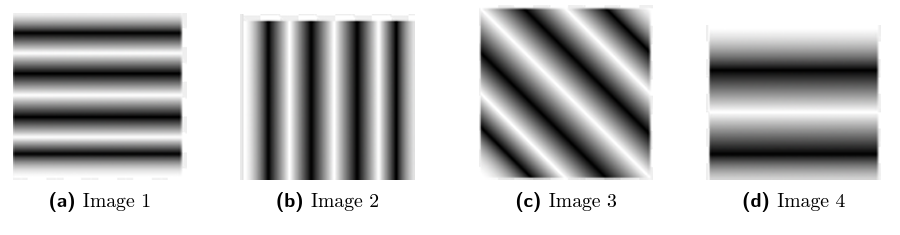
\includegraphics[width=0.8\textwidth]{sinusodial_gratings.png}
    \caption{Determining Position}
    \label{fig:2.3.3}
\end{figure}
as mentiond above , the $k_x$ coordinate represents the spatial frequency in the horizontal direction. Therefore each sinusodial gratings that is only in the horizontal direction has a $k_x$ component based on its freqeuncy. In the map there is only one point with only $k_x$ component and it corresponds to the image 2.
The same goes for the $k_y$ component and the vertical sinusodial gratings. The points with only $k_y$ component corresponds to the image 1 and 4, and beacuse the frequenct of image 1 is higher the point with higher magnitude on the y axis is for the image 1 and the other one on the y axis is for the image 4. This leaves the image 3 for the point with both $k_x$ and $k_y$ components, which makes sense beacuse rotating in the k-space is equivalent to rotating the image in the spatial domain.
\begin{figure}[H]
    \centering
    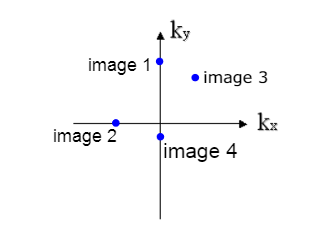
\includegraphics[width=0.6\textwidth]{k_space.png}
    \caption{Determining Position}
    \label{fig:2.3.3}
\end{figure}
\subsection{2.3.4 Low Pass and High Pass Filters}
If we delete the high frequency components from the k-space, we are essentially removing the high frequency components from the image. This is equivalent to applying a low pass filter to the image. By applying a low pass filter not very much power is being thrown away beyond the sqaure that is cut off. If we were to reconstrcute the image after deleting the high-frequencies , we would see that the image is blurry and the edges are not sharp, but the overall contrast would still be pretty good due to the fact that not too much power was thrown away.
\\
Now if we were to apply a high pass filter to the image , that is removing the low frequency components from the image, we would see that the image is very blurry and the contrast is very low. This is because the low frequency components are the ones that carry the most power and by removing them we are throwing away a lot of power. This time the image will look completely black and empty, but in fact it is not empty , and the filter has preserved the image information where there are very rapid changes in the gray level. Such a process is frequently desired in an edge detector.
\begin{figure}[H]
    \centering
    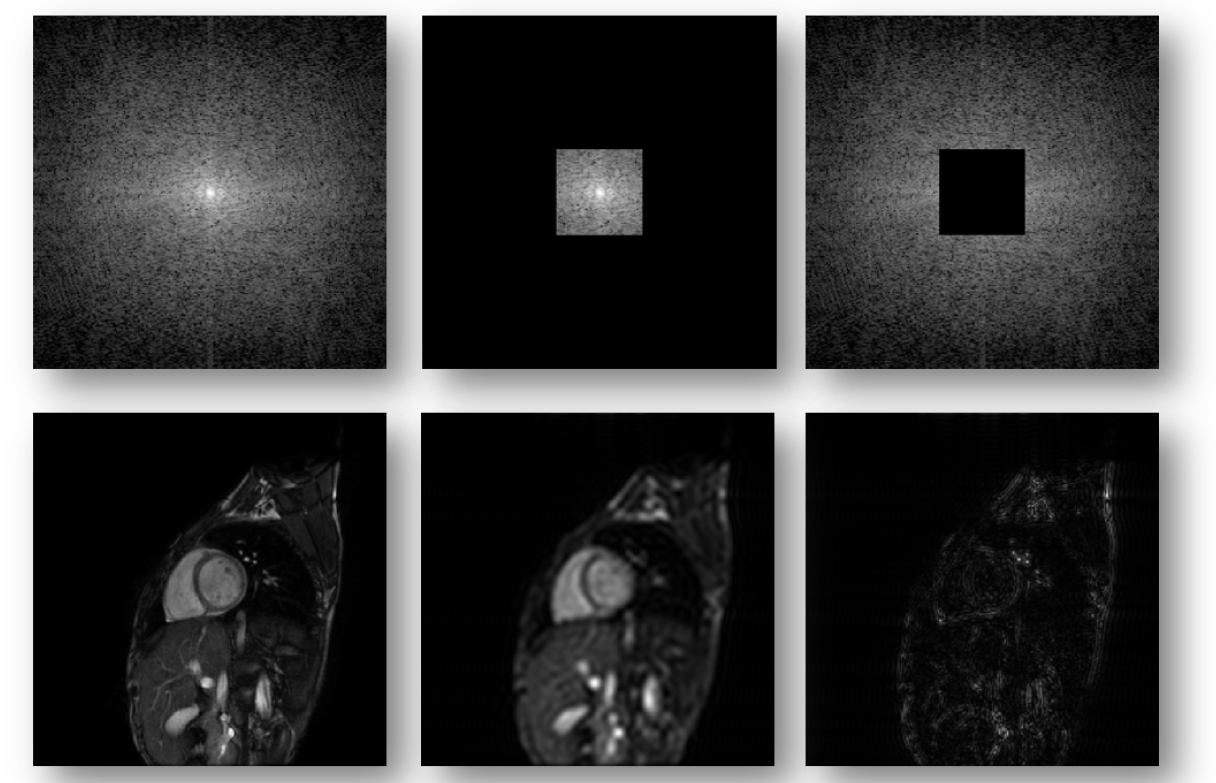
\includegraphics[width=0.6\textwidth]{high_low_filter_one.png}
    \caption{After result of applying low pass and high pass filters to the image}
    \label{fig:2.3.3}
\end{figure}
\section{3.1 MRI reconstruction methods}
\subsection{3.1.1 Filtered Back Projection}
Filtered back projection (FBP) is a reconstruction technique commonly used in computed tomography (CT) to convert X-ray projection data into a 2D or 3D image of an object. This process includes several key steps:
\begin{itemize}
\item Data Collection: X-ray measurements are collected from multiple angles as the X-ray source rotates around the object. These measurements, called projections, show how much x-rays are attenuated as they pass through an object.
\item Preprocessing: Raw projection data is often preprocessed to improve certain features and reduce artifacts. An important step in preprocessing is filtering, in which the data is subjected to a mathematical filtering operation. A popular choice is the application of a ramp filter.
\item Filtered data: The filtering step is necessary to improve the quality of the reconstructed image. It amplifies higher frequency components in the data, thus providing sharper images. The filtered data is then used in the reconstruction process.
\item Back projection: The core of the FBP algorithm is back projection. In this step, the filtered projection data is mathematically transformed to reconstruct the original image. Each point in the reconstructed image corresponds to the contribution of several rays from different angles.
\item Reconstruction Algorithm: FBP exploits the principles of Radon transform and inverse Radon transform to perform accurate back projection. The algorithm takes into account the geometry of the imaging system and uses mathematical operations to reconstruct the spatial distribution of X-ray attenuation in the object.
\item Fourier transform: FBP often involves the use of Fourier transform. The filtered projection data is converted to the frequency domain using Fourier analysis, allowing efficient application of filtering and subsequent back-projection.

\item Final image: The result of the FBP algorithm is a reconstructed image that represents the distribution of X-ray attenuation coefficients in the imaged object. This image provides valuable information about an object's internal structure, making it a powerful tool in medical imaging, industrial non-destructive testing, and other applications.
\end{itemize}
 Filtered back projection is known for its computational efficiency and is widely used in practical CT imaging. However, it may have limitations in handling noisy or incomplete data. Advanced iterative reconstruction methods have been developed to address some of these challenges, but FBP remains a fundamental and widely used technique in tomographic image reconstruction.
\subsection{3.1.2 Compressed Sensing}
Compressed sensing (also known as compressive sensing, compressive sampling, or sparse sampling) is a signal processing technique for efficiently acquiring and reconstructing a signal, by finding solutions to underdetermined linear systems. This is based on the principle that, through optimization, the sparsity of a signal can be exploited to recover it from far fewer samples than required by the Nyquist–Shannon sampling theorem. There are two conditions under which recovery is possible. The first one is sparsity, which requires the signal to be sparse in some domain. The second one is incoherence, which is applied through the isometric property, which is sufficient for sparse signals. Compressed sensing has applications in, for example, MRI where the incoherence condition is typically satisfied.
\section{3.2 Questions}
\subsection{3.2.3 Reconstructing the MRI}
After loading the data in the rawkneedata.mat file, we then reconstruct the final image using the inverse fast fourier transform function in matlab.
Remeber to apply fftshift also after the inverse Fourier transform. Matlab assumes that the low frequencies are in the 'top left' corner of your matrix. If you ignore this, your phase information will be wrong. In the kSpace you show, kSpace center is actually in the middle of the matrix.
\subsection{3.2.4 the MRI Image}
\begin{figure}[H]
    \centering
    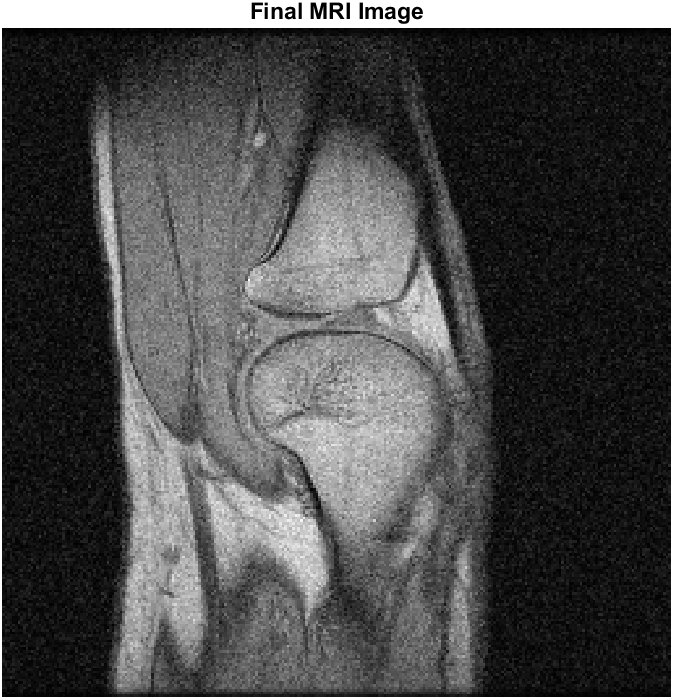
\includegraphics[width=0.55\textwidth]{knee_mri.png}
    \caption{MRI Image}
    \label{fig:2.3.3}
\end{figure}
one small detail is that the image is flipped vertically, but that is not a problem. Normally the Femur bone is on the top.
\subsection{3.2.5 Noises in medical imaging}

Noise in medical imaging refers to unwanted variations or disturbances in an image that can affect the accuracy and quality of the diagnostic information. Various types of noise can arise from different sources throughout the process of medical image acquisition, processing, and display. Understanding and managing noise are critical aspects of maintaining image quality and improving the reliability of diagnostic information. Here are some common types of noise in medical imaging:
\begin{itemize}
    \item Electronic Noise: Electronic noise is introduced during the signal readout and processing stages in the imaging system. It includes thermal noise from electronic components, amplifier noise, and other electronic artifacts. Electronic noise can contribute to fluctuations in pixel values and degrade image quality.
    \item Reconstruction Artifacts: In computed tomography (CT) and other tomographic imaging modalities, errors in image reconstruction algorithms can result in artifacts. Ring artifacts, streak artifacts, and shading artifacts are examples of reconstruction-related noise.
    \item Radiofrequency Interference (RFI): In magnetic resonance imaging (MRI), external electromagnetic interference, such as radiofrequency interference, can introduce noise and affect image quality. Shielding and proper RF filtering are essential to minimize RFI.
\end{itemize}
Gaussian noise and Impulse noise are popular noises distributed in magnitude MR images and non-avoidable
\section{4.1 Histogram}
Here we can see the Histogram of the noiseless and noisey image side by side.
\begin{figure}[H]
	\centering
	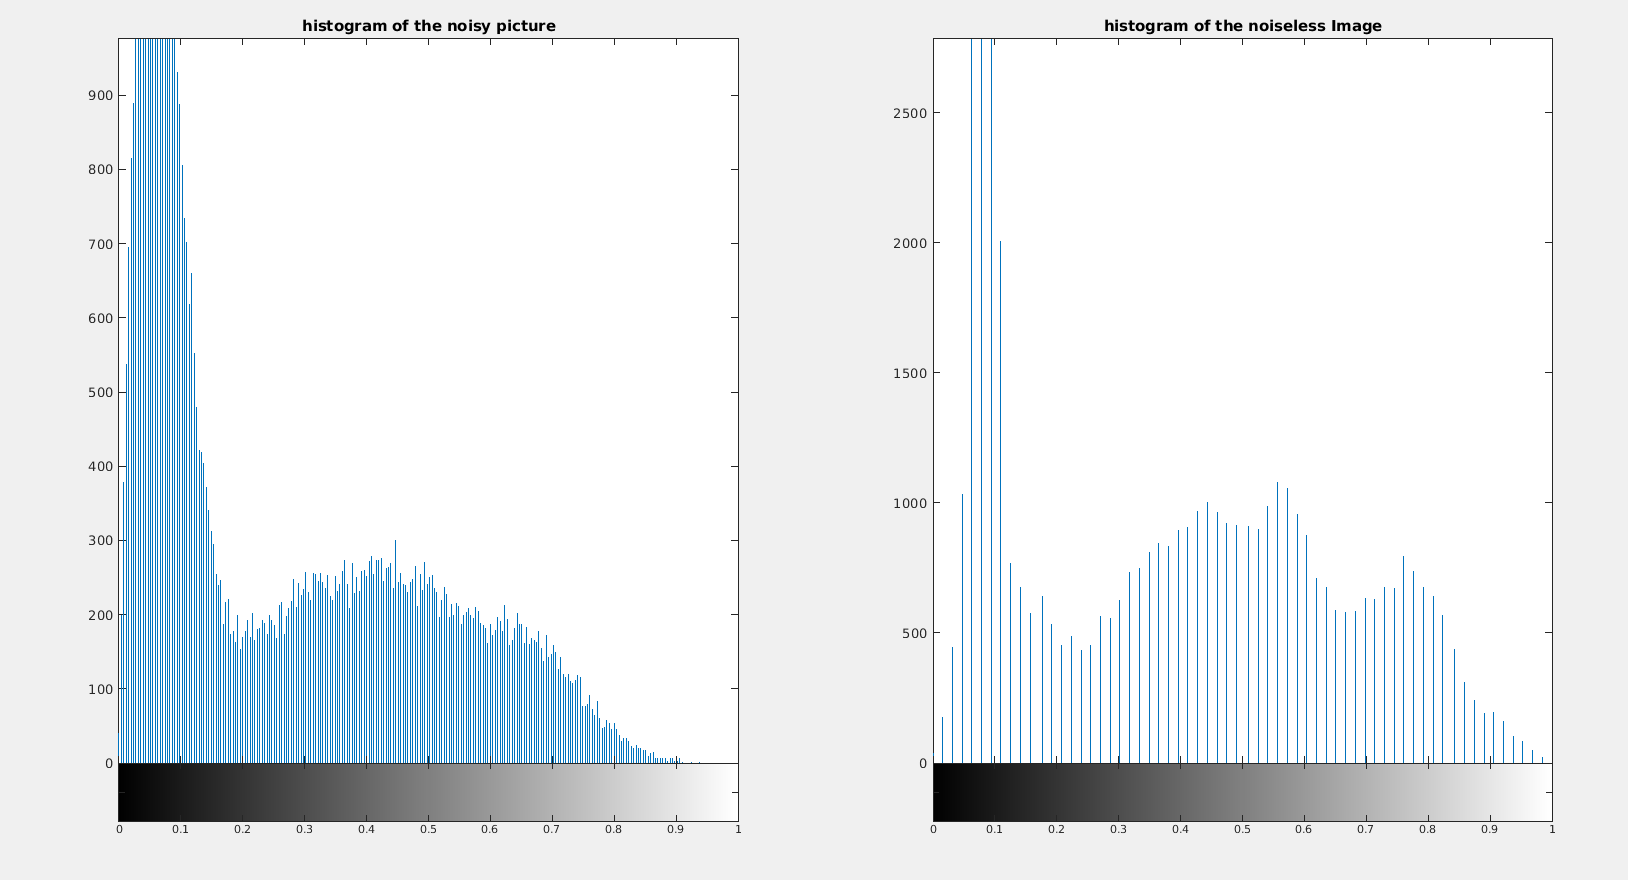
\includegraphics[width=0.95\textwidth]{histogram.png}
	\caption{Histogram of the Images}
	\label{fig:2.3.3}
\end{figure}
\newpage
\section{4.2 Low Pass Filters}
\subsection{Mean Filter}
mean filter is one of the techniques which is used to reduce noise of the images.\\
This is a local averaging operation and it is a one of the simplest linear filter. The value of each pixel is replaced by the average of all the values in the local neighborhood. Let f(i,j) is a noisy image then the smoothed image g(x,y) can be obtained by,
\begin{figure}[H]
	\centering
	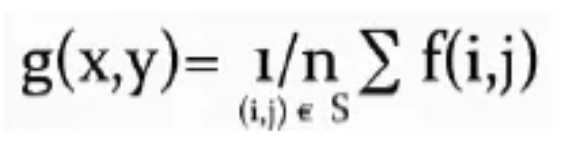
\includegraphics[width=0.35\textwidth]{meanfilterformula.png}
	\caption{Mean filter}
	\label{fig:2.3.3}
\end{figure}
\subsection{Median Filter}
Median Filter is one of Non-linear filters, which is also used for smoothing. Its basic idea is to replace each pixel by the median of its neighboring pixels.\\
By doing so, it removes some spikes introduced by noise: especially impulse and salt and pepper noise. This is because stand-alone noise pixels with extreme intensities like black and white cannot survive after median filtering. Another advantage of median filter is that it does not introduce new pixel values since it only re-use exisiting pixel values from window. Further, unlike other averaging filters, it remove noise without losing edge information.
\subsection{Gaussian Filter}
Gaussian kernel, as its name implies, has the shape of the function ‘Gaussian distribution’ to define the weights inside the kernel, which are used to compute the weighted average of the neighboring points (pixels) in an image.\\
In other words, each value in the Gaussian filter is from the zero mean Gaussian distribution. One thing we need to keep in mind is that the kernel size is dependent of standard deviation $\sigma$ of Gaussian function.
\section{4.3 Mean Filter}
the function that we have written looks like this :
\lstinputlisting{mean.m}
It's a Mean filter with a 3*3 kernel. Here is the result of applying the filter on the image that we reconstructed in the 3rd part.
\begin{figure}[H]
	\centering
	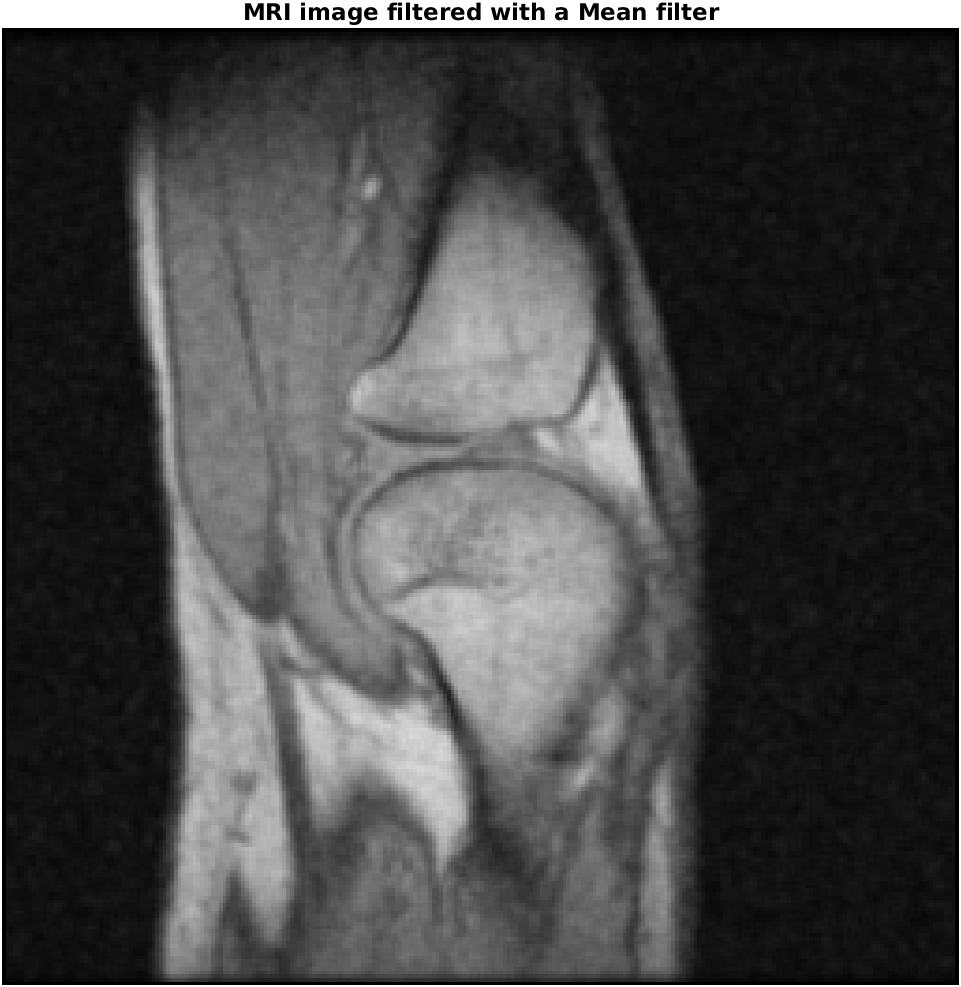
\includegraphics[width=0.75\textwidth]{meanFilteredImage.png}
	\caption{Mean filtered Image}
	\label{fig:2.3.3}
\end{figure}
\section{4.4 Median Filter}
We use the pre-built function medfilt2 in matlab.
\lstinputlisting{median.m}
and the output of this function is as follows :
\begin{figure}[H]
	\centering
	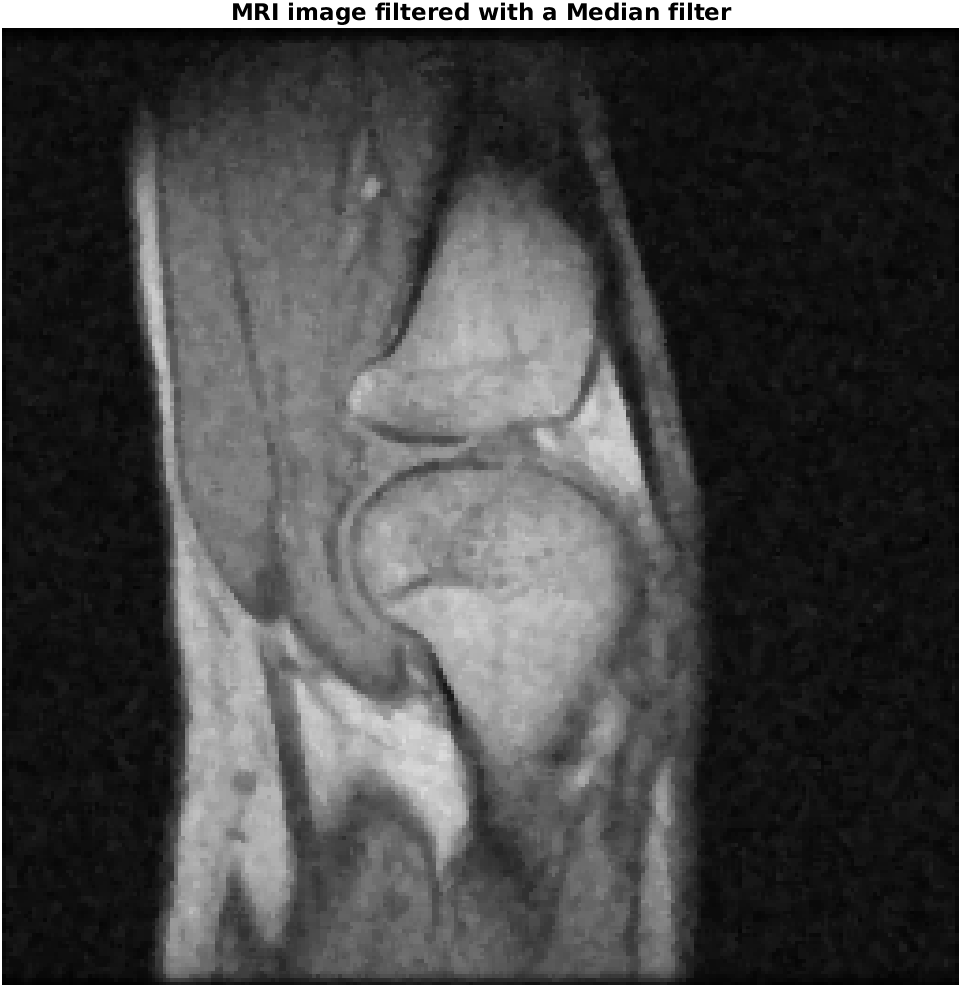
\includegraphics[width=0.75\textwidth]{medianFilteredImage.png}
	\caption{Median filter}
	\label{fig:2.3.3}
\end{figure}
\section{4.5 Gaussian Filter}
Since we are not allowed to use any prebuilt Gaussian Function , the written Gaussian function is as follows :
\lstinputlisting{gaussian.m}
Here's the after results :
\begin{figure}[H]
	\centering
	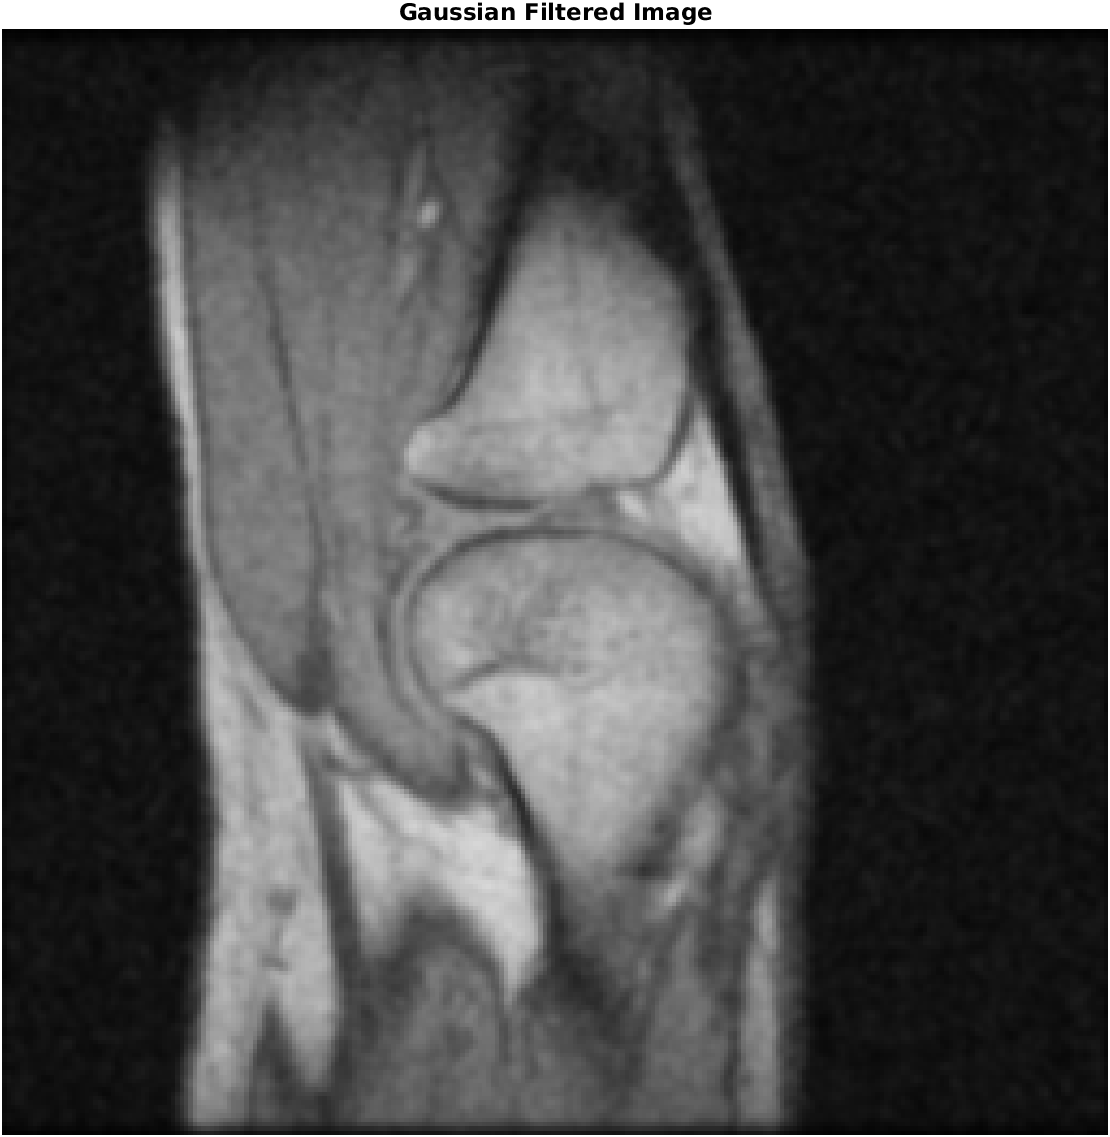
\includegraphics[width=0.75\textwidth]{gaussianFilteredimage.png}
	\caption{Gaussian filter}
	\label{fig:2.3.3}
\end{figure}
\section{4.6 NLM filter}
Non-local means is an algorithm in image processing for image denoising. Unlike "local mean" filters, which take the mean value of a group of pixels surrounding a target pixel to smooth the image, non-local means filtering takes a mean of all pixels in the image, weighted by how similar these pixels are to the target pixel. This results in much greater post-filtering clarity, and less loss of detail in the image compared with local mean algorithms.\\
For working with this filter , we use the pre-built imnlmfilt in matlab. The output is as follows :
\begin{figure}[H]
	\centering
	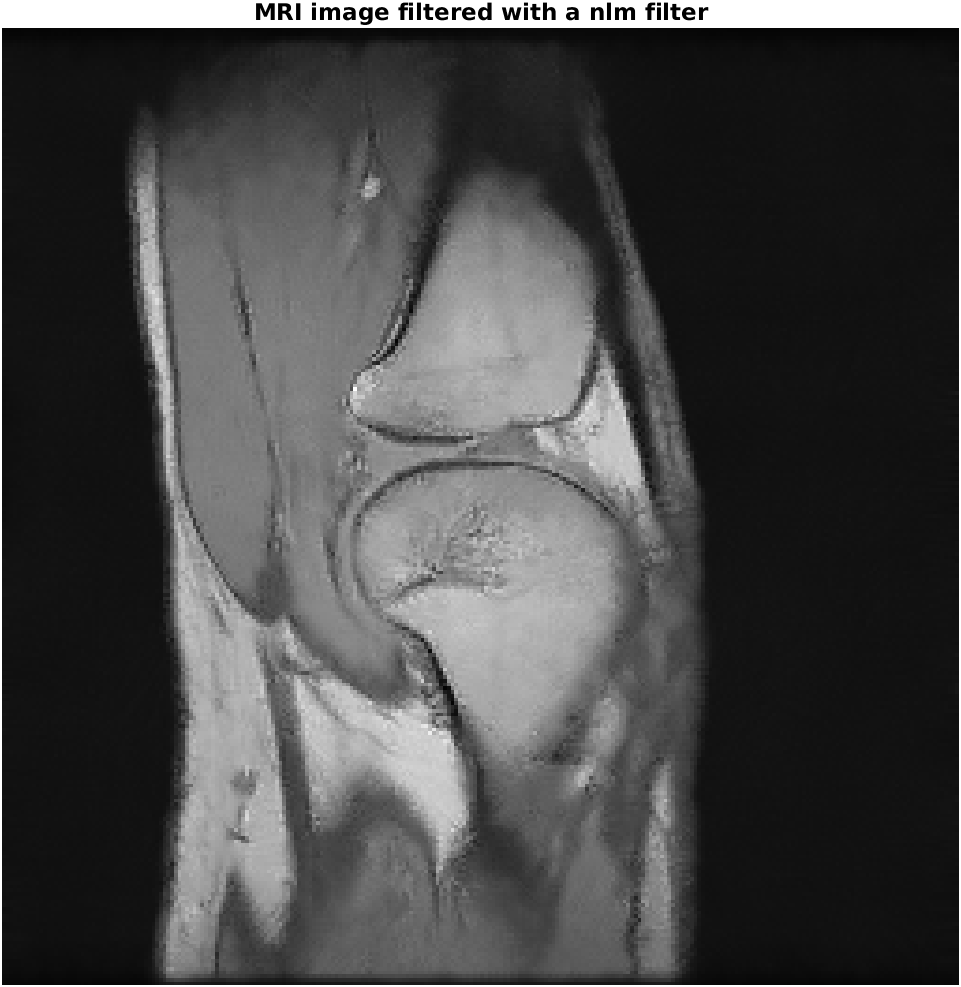
\includegraphics[width=0.75\textwidth]{nlmfilter.png}
	\caption{Non-Local-Means filter}
	\label{fig:2.3.3}
\end{figure}
\section{4.7 SNR and PSNR Results}
Signal-to-noise ratio (SNR or S/N) is a measure used in science and engineering that compares the level of a desired signal to the level of background noise. SNR is defined as the ratio of signal power to noise power, often expressed in decibels. A ratio higher than 1:1 (greater than 0 dB) indicates more signal than noise.\\
Peak signal-to-noise ratio (PSNR) is an engineering term for the ratio between the maximum possible power of a signal and the power of corrupting noise that affects the fidelity of its representation. Because many signals have a very wide dynamic range, PSNR is usually expressed as a logarithmic quantity using the decibel scale. \\
Here is the SNR and PSNR Table for comparing the output of each of the defined filters with the noiseless image kneeMRI.jpg which was in the project folder.
\begin{figure}[H]
	\centering
	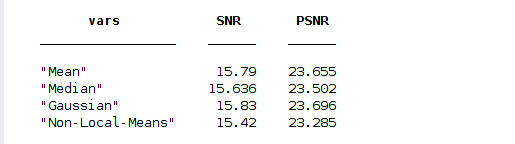
\includegraphics[width=0.95\textwidth]{snr_psnr.png}
	\caption{Evaluation}
	\label{fig:2.3.3}
\end{figure}
The results don't differ a lot, but the best SNR and PSNR values belong to Gaussian.
\end{document}